\documentclass{article}


\usepackage{tikz,latexsym}



\usetikzlibrary{arrows,decorations.pathmorphing,decorations.pathreplacing,backgrounds,positioning,fit,matrix}
\usetikzlibrary{shapes,calc,patterns,arrows.meta}
\tikzset{
	vert/.style={circle,inner sep=1.5,fill=white,draw,minimum size=.3cm},
	edge/.style={color=black, thick},
	diredge/.style={->,>={Stealth[width=8pt,length=8pt]},color=black, thick},
	timelabel/.style={fill=white,font=\footnotesize, text centered},
	wave/.style={decorate,decoration={coil,aspect=0}},
	dirwave/.style={->, >={Stealth[width=8pt,length=8pt]},decorate,decoration={coil,aspect=0}},
	diredge2/.style={->,>={Stealth[width=8pt,length=8pt]}}
}
%\tikzstyle{wave} = [decorate,decoration={coil,aspect=0}]
%\tikzstyle{dirwave} = [-{Latex[length=2.5mm]},decorate,decoration={coil,aspect=0}]
%\tikzstyle{diredge2} = [-{Latex[length=2.5mm]}]

\usepackage{caption} %for subfigure - join multiple figures and add captions
\usepackage{subcaption}

\begin{document}
\begin{figure}
	\centering
	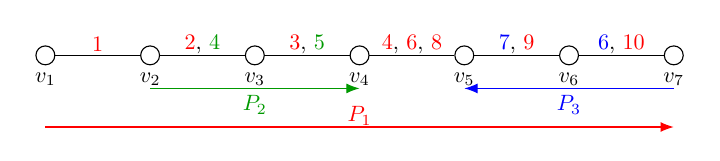
\begin{tikzpicture}[scale = 0.7, every node/.style={scale=0.8},xscale=.95]
		% Variables for distances 
		\def\x{2} % Nodes are \x apart
		\def\y{0.2} % Labels are at distance 0.5 * \x between nodes and \y vertically from the line
		\def\gr{green!60!black}
		\def\bl{blue}
		\def\rd{red}
		
		\node[vert,label=below:$v_1$] (V1) at (1,0) {};
		\node[vert,label=below:$v_2$] (V2) at ($ (V1) + \x*(1,0)$) {};
		\node[vert,label=below:$v_3$] (V3) at ($ (V2) + \x*(1,0)$) {};
		\node[vert,label=below:$v_4$] (V4) at ($ (V3) + \x*(1,0)$) {};
		\node[vert,label=below:$v_5$] (V5) at ($ (V4) + \x*(1,0)$) {};
		\node[vert,label=below:$v_6$] (V6) at ($ (V5) + \x*(1,0)$) {};
		\node[vert,label=below:$v_7$] (V7) at ($ (V6) + \x*(1,0)$) {};
		
		\path[draw] (V1) --(V2);
		\node at ($ (V1) + 0.5*\x*(1,0) + \y*(0,1)$) {{\color{\rd}$1$}};
		\path[draw] (V2) --(V3);
		\node at ($ (V2) + 0.5*\x*(1,0) + \y*(0,1)$) {{\color{\rd}$2$}, {\color{\gr}$4$}};
		\path[draw] (V3) --(V4);
		%\node at ($ (V3) + 0.5*\x*(1,0) + \y*(0,1)$) {{\color{\rd}$3$}, {\color{\gr}$5$},  {\color{\rd}$6$}};
		\node at ($ (V3) + 0.5*\x*(1,0) + \y*(0,1)$) {{\color{\rd}$3$}, {\color{\gr}$5$}};
		\path[draw] (V4) --(V5);
		%\node at ($ (V4) + 0.5*\x*(1,0) + \y*(0,1)$) {{\color{\rd}$4$}, {\color{\rd}$8$}};
		\node at ($ (V4) + 0.5*\x*(1,0) + \y*(0,1)$) {{\color{\rd}$4$}, {\color{\rd}$6$}, {\color{\rd}$8$}};
		
		\path[draw] (V5) --(V6);
		%\node at ($ (V5) + 0.5*\x*(1,0) + \y*(0,1)$) {{\color{\bl}$6$}, {\color{\rd}$9$}};
		\node at ($ (V5) + 0.5*\x*(1,0) + \y*(0,1)$) {{\color{\bl}$7$}, {\color{\rd}$9$}};
		\path[draw] (V6) --(V7);
		%\node at ($ (V6) + 0.5*\x*(1,0) + \y*(0,1)$) {{\color{\bl}$5$}, {\color{\rd}$10$}};
		\node at ($ (V6) + 0.5*\x*(1,0) + \y*(0,1)$) {{\color{\bl}$6$}, {\color{\rd}$10$}};
		
		%\draw[->] ($ (V1) + 2 * \yy * (0,1)$) -- ($ (V7) + 2 * \yy * (0,1)$);
		
		\draw[-Latex,color=\rd] ($(V1) - (0,1.3)$) -- ($ (V7) - (0,1.3)$);
		\node at ($(V4) -(0,1.1)$) {\color{\rd}$P_1$} {};
		\draw[-Latex,color=\gr] ($(V2) - (0,0.6)$) -- ($ (V4) - (0,0.6)$);
		\node at ($(V3) -(0,0.9)$) {\color{\gr}$P_2$} {};
		\draw[-Latex,color=\bl] ($(V7) - (0,0.6)$) -- ($ (V5) - (0,0.6)$);
		\node at ($(V6) -(0,0.9)$) {\color{\bl}$P_3$} {};
		
	\end{tikzpicture}
	\caption{}
	\label{fig:}
\end{figure}

	%%G1
	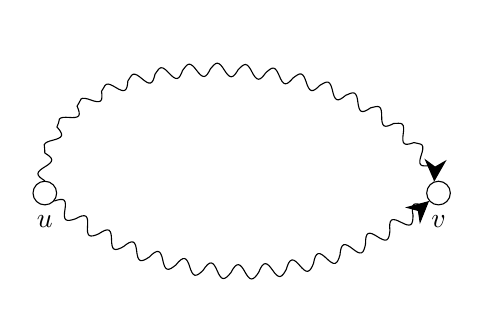
\begin{tikzpicture}
		\node[vert,label=below:$u$] (u) at (1,0) {};
		\node[vert,label=below:$v$] (v) at (6,0) {};
		
		\draw [dirwave] (u) to [out=90,in=110] (v);
		\draw [dirwave] (u) to [out=320,in=220] (v);
		
	\end{tikzpicture}

	%%G2
	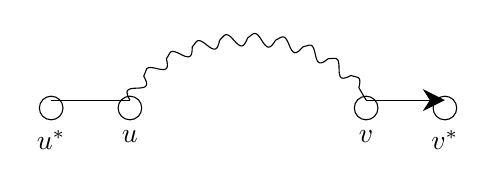
\begin{tikzpicture}
		\node[vert,label=below:$u^*$] (u*) at (1,0) {};
		\node[vert,label=below:$u$] (u) at (2,0) {};
		\node[vert,label=below:$v$] (v) at (5,0) {};
		\node[vert,label=below:$v^*$] (v*) at (6,0) {};
		
		%\draw (u*) -- (u) (v*) -- (v);
		
		%\draw [wave] (u*) to [out=320,in=220] (v*);
		\draw [transform canvas={yshift=1mm}] 
		(1,0) -- (2,0) 
		(2,0) edge[wave] [out=60,in=120] (5,0) 
		(5,0) edge[diredge2] (6,0);
		
	\end{tikzpicture}

	%%G4
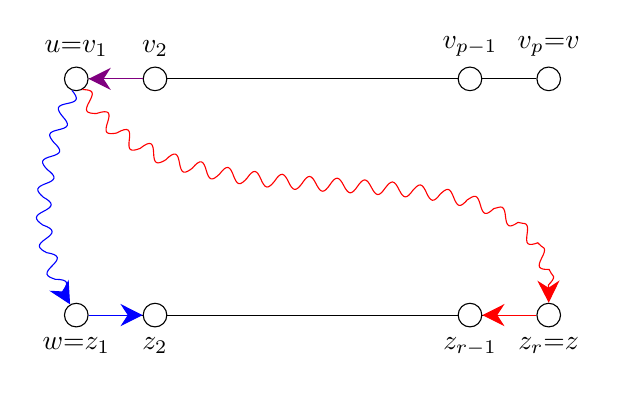
\begin{tikzpicture}
	%%%S_uv
\node[vert,label=above:$u {=} v_1$] (v1) at (1,0) {};
\node[vert,label=above:$v_2$] (v2) at (2,0) {};
\node[vert,label=above:$v_{p-1}$] (vp1) at (6,0) {};
\node[vert,label=above:$v_p {=} v$] (vp) at (7,0) {};
\draw (v1) -- (v2) -- (vp1) -- (vp);

%%%% S_wz
\node[vert,label=below:$w {=} z_1$] (z1) at (1,-3) {};
\node[vert,label=below:$z_2$] (z2) at (2,-3) {};
\node[vert,label=below:$z_{r-1}$] (zr1) at (6,-3) {};
\node[vert,label=below:$z_r {=} z$] (zr) at (7,-3) {};
\draw (z1) -- (z2) -- (zr1) -- (zr);


\draw [violet] (v2) edge[diredge2] (v1);

\draw [blue]%[transform canvas={yshift=0.5mm},thick] 
(v1) edge[dirwave] [out=250,in=120] (z1) 
(z1) edge[diredge2] (z2);


\draw [red] %[transform canvas={yshift=-0.5mm}] 
(v1) edge[dirwave] [out=300,in=90] (zr) 
(zr) edge[diredge2] (zr1);
\end{tikzpicture}

	%%G5
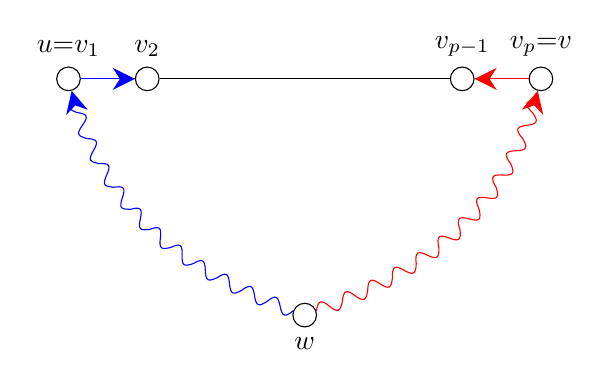
\begin{tikzpicture}
	%%%S_uv
	\node[vert,label=above:$u {=} v_1$] (v1) at (1,0) {};
	\node[vert,label=above:$v_2$] (v2) at (2,0) {};
	\node[vert,label=above:$v_{p-1}$] (vp1) at (6,0) {};
	\node[vert,label=above:$v_p {=} v$] (vp) at (7,0) {};
	\draw (v1) -- (v2) -- (vp1) -- (vp);
	
	%%%% node w
	\node[vert,label=below:$w$] (w) at (4,-3) {};
	
	
	
	\draw [blue]%[transform canvas={yshift=0.5mm},thick] 
	(w) edge[dirwave] [out=160,in=285] (v1) 
	(v1) edge[diredge2] (v2);
	
	\draw [red]%[transform canvas={yshift=0.5mm},thick] 
	(w) edge[dirwave] [out=20,in=255] (vp) 
	(vp) edge[diredge2] (vp1);
	
	
\end{tikzpicture}

	%%G6
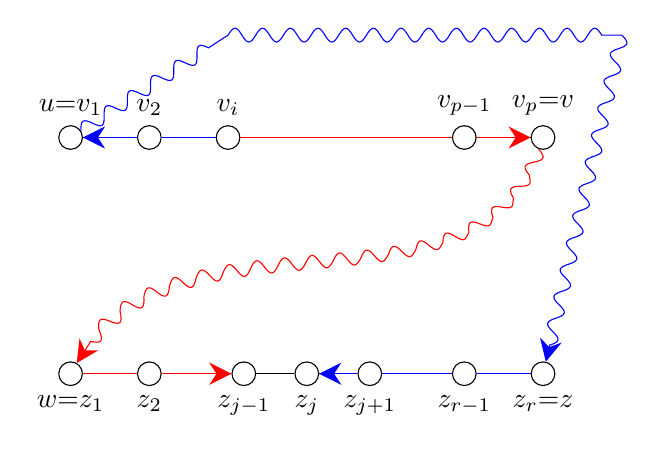
\begin{tikzpicture}
	%%%S_uv
	\node[vert,label=above:$u {=} v_1$] (v1) at (1,0) {};
	\node[vert,label=above:$v_2$] (v2) at (2,0) {};
	\node[vert,label=above:$v_i$] (vi) at (3,0) {};
	\node[vert,label=above:$v_{p-1}$] (vp1) at (6,0) {};
	\node[vert,label=above:$v_p {=} v$] (vp) at (7,0) {};
	\draw (v1) -- (v2) -- (vi) -- (vp1) -- (vp);
	
	%%%% S_wz
	\node[vert,label=below:$w {=} z_1$] (z1) at (1,-3) {};
	\node[vert,label=below:$z_2$] (z2) at (2,-3) {};
	\node[vert,label=below:$z_{j-1}$] (zj-1) at (3.2,-3) {};
	\node[vert,label=below:$z_{j}$] (zj) at (4,-3) {};
	\node[vert,label=below:$z_{j+1}$] (zj+1) at (4.8,-3) {};
	\node[vert,label=below:$z_{r-1}$] (zr1) at (6,-3) {};
	\node[vert,label=below:$z_r {=} z$] (zr) at (7,-3) {};
	\draw (z1) -- (z2) -- (zj-1) -- (zj) -- (zj+1) -- (zr1) -- (zr);
	
	
	
	\draw [blue]%[transform canvas={yshift=0.5mm},thick] 
	(vi) -- (v2) edge[diredge2] (v1) 
	(v1) edge[wave] (3,1.3) 
	(3,1.3) edge[wave] (8,1.3)
	(8,1.3) edge[dirwave] (zr) 
	(zr) --(zr1) -- (zj+1)
	(zj+1) edge[diredge2] (zj);
	
	\draw [red]
	(vi) -- (vp1) edge[diredge2] (vp) 
	(vp) edge[dirwave] [out=250,in=60] (z1) 
	(z1) --(z2)
	(z2) edge[diredge2] (zj-1);
	

\end{tikzpicture}

	%%G7
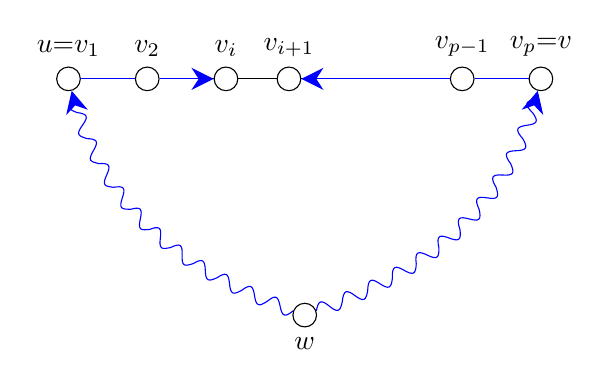
\begin{tikzpicture}
	%%%S_uv
	\node[vert,label=above:$u {=} v_1$] (v1) at (1,0) {};
	\node[vert,label=above:$v_2$] (v2) at (2,0) {};
	\node[vert,label=above:$v_i$] (vi) at (3,0) {};
	\node[vert,label=above:$v_{i+1}$] (vi+1) at (3.8,0) {};
	\node[vert,label=above:$v_{p-1}$] (vp1) at (6,0) {};
	\node[vert,label=above:$v_p {=} v$] (vp) at (7,0) {};
	\draw (v1) -- (v2) -- (vi) -- (vi+1) -- (vp1) -- (vp);
	
	%%%% node w
	\node[vert,label=below:$w$] (w) at (4,-3) {};
	
	
	
	\draw [blue] 
	(w) edge[dirwave] [out=160,in=285] (v1) 
	(v1) -- (v2)
	(v2) edge[diredge2] (vi);
	
	\draw [blue]
	(w) edge[dirwave] [out=20,in=255] (vp) 
	(vp) -- (vp1)
	(vp1) edge[diredge2] (vi+1);
	
	
\end{tikzpicture}

	%%G8
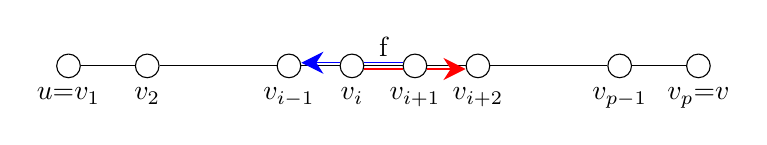
\begin{tikzpicture}
	%%%S_uv
	\node[vert,label=below:$u {=} v_1$] (v1) at (1,0) {};
	\node[vert,label=below:$v_2$] (v2) at (2,0) {};
	\node[vert,label=below:$v_{i-1}$] (vi-1) at (3.8,0) {};
	\node[vert,label=below:$v_{i}$] (vi) at (4.6,0) {};
	\node[vert,label=below:$v_{i+1}$] (vi+1) at (5.4,0) {};
	\node[vert,label=below:$v_{i+2}$] (vi+2) at (6.2,0) {};
	\node[vert,label=below:$v_{p-1}$] (vp1) at (8,0) {};
	\node[vert,label=below:$v_p {=} v$] (vp) at (9,0) {};
	\draw (v1) -- (v2)  -- (vi-1) -- (vi) -- (vi+1) -- (vi+2) -- (vp1) -- (vp);
	\path (vi) -- (vi+1) node [midway,above] {f};	
	
	
	
	\draw [blue,transform canvas={yshift=0.4mm}] 
	(vi+1) -- (vi)
	(vi) edge[diredge2] (vi-1);
	
	\draw [red,transform canvas={yshift=-0.4mm}] 
	(vi) -- (vi+1)
	(vi+1) edge[diredge2] (vi+2);
	

	
	
\end{tikzpicture}

\clearpage

\begin{figure}[h]
	\centering
	\begin{subfigure}[b]{0.48\textwidth}
		\centering
		\resizebox{\linewidth}{!}{
			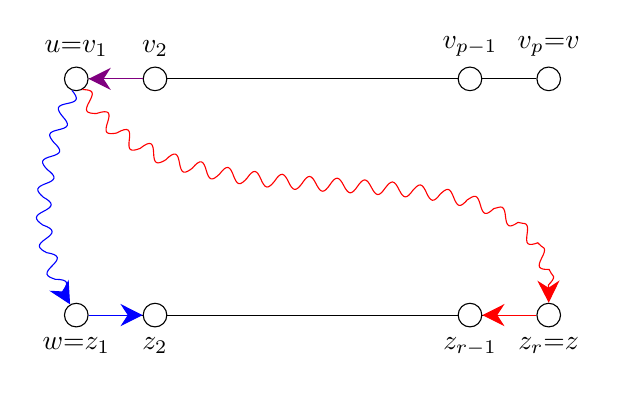
\begin{tikzpicture}
				%%%S_uv
				\node[vert,label=above:$u {=} v_1$] (v1) at (1,0) {};
				\node[vert,label=above:$v_2$] (v2) at (2,0) {};
				\node[vert,label=above:$v_{p-1}$] (vp1) at (6,0) {};
				\node[vert,label=above:$v_p {=} v$] (vp) at (7,0) {};
				\draw (v1) -- (v2) -- (vp1) -- (vp);
				
				%%%% S_wz
				\node[vert,label=below:$w {=} z_1$] (z1) at (1,-3) {};
				\node[vert,label=below:$z_2$] (z2) at (2,-3) {};
				\node[vert,label=below:$z_{r-1}$] (zr1) at (6,-3) {};
				\node[vert,label=below:$z_r {=} z$] (zr) at (7,-3) {};
				\draw (z1) -- (z2) -- (zr1) -- (zr);
				
				
				\draw [violet] (v2) edge[diredge2] (v1);
				
				\draw [blue]%[transform canvas={yshift=0.5mm},thick] 
				(v1) edge[dirwave] [out=250,in=120] (z1) 
				(z1) edge[diredge2] (z2);
				
				
				\draw [red] %[transform canvas={yshift=-0.5mm}] 
				(v1) edge[dirwave] [out=300,in=90] (zr) 
				(zr) edge[diredge2] (zr1);
		\end{tikzpicture}}
		\caption{Example of a guess G-4, where we guessed the fastest temporal paths of form $v_2 \rightarrow u \leadsto w \rightarrow z_2$ (in blue)
			and $v_2 \rightarrow u \leadsto z \rightarrow z_{r-1}$ (in red).
			\label{fig:FPT-guessG4}}
	\end{subfigure}
	\quad
	\begin{subfigure}[b]{0.48\textwidth}
		\centering
		\resizebox{\linewidth}{!}{
			
			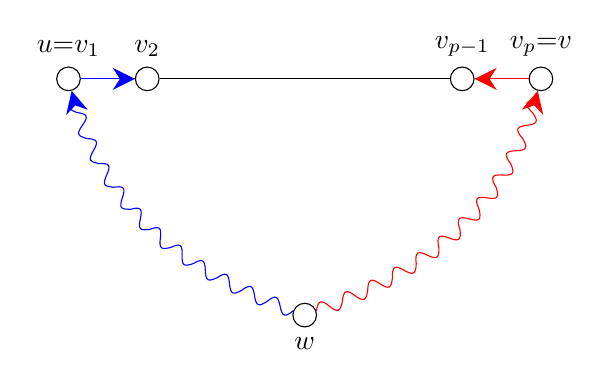
\begin{tikzpicture}
				%%%S_uv
				\node[vert,label=above:$u {=} v_1$] (v1) at (1,0) {};
				\node[vert,label=above:$v_2$] (v2) at (2,0) {};
				\node[vert,label=above:$v_{p-1}$] (vp1) at (6,0) {};
				\node[vert,label=above:$v_p {=} v$] (vp) at (7,0) {};
				\draw (v1) -- (v2) -- (vp1) -- (vp);
				
				%%%% node w
				\node[vert,label=below:$w$] (w) at (4,-3) {};
				
				
				
				\draw [blue]%[transform canvas={yshift=0.5mm},thick] 
				(w) edge[dirwave] [out=160,in=285] (v1) 
				(v1) edge[diredge2] (v2);
				
				\draw [red]%[transform canvas={yshift=0.5mm},thick] 
				(w) edge[dirwave] [out=20,in=255] (vp) 
				(vp) edge[diredge2] (vp1);
				
				
		\end{tikzpicture}}
		\caption{Example of a guess G-5, where we guessed the fastest temporal paths of form $w \leadsto u \rightarrow v_2$ (in blue) and $w \leadsto v \rightarrow v_{p-1}$ (in red). 
			\label{fig:FPT-guessG5}}
	\end{subfigure}
	
	\begin{subfigure}[b]{0.48\textwidth}
		\centering
		\resizebox{1.2\linewidth}{!}{
			%
			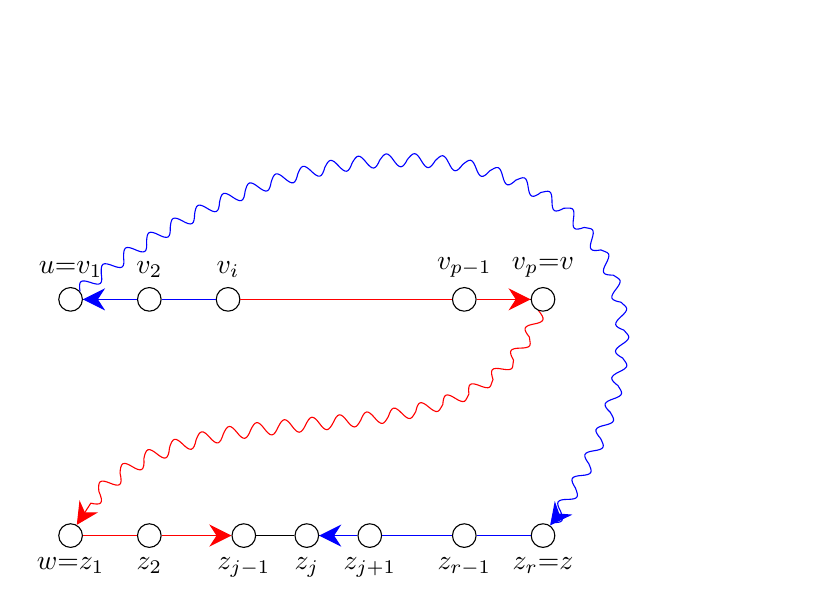
\begin{tikzpicture}[scale=1]
				%%%S_uv
				\node[vert,label=above:$u {=} v_1$] (v1) at (1,0) {};
				\node[vert,label=above:$v_2$] (v2) at (2,0) {};
				\node[vert,label=above:$v_i$] (vi) at (3,0) {};
				\node[vert,label=above:$v_{p-1}$] (vp1) at (6,0) {};
				\node[vert,label=above:$v_p {=} v$] (vp) at (7,0) {};
				\draw (v1) -- (v2) -- (vi) -- (vp1) -- (vp);
				
				%%%% S_wz
				\node[vert,label=below:$w {=} z_1$] (z1) at (1,-3) {};
				\node[vert,label=below:$z_2$] (z2) at (2,-3) {};
				\node[vert,label=below:$z_{j-1}$] (zj-1) at (3.2,-3) {};
				\node[vert,label=below:$z_{j}$] (zj) at (4,-3) {};
				\node[vert,label=below:$z_{j+1}$] (zj+1) at (4.8,-3) {};
				\node[vert,label=below:$z_{r-1}$] (zr1) at (6,-3) {};
				\node[vert,label=below:$z_r {=} z$] (zr) at (7,-3) {};
				\draw (z1) -- (z2) -- (zj-1) -- (zj) -- (zj+1) -- (zr1) -- (zr);
				
				
				
				\draw [blue]%[transform canvas={yshift=0.5mm},thick] 
				(vi) -- (v2) edge[diredge2] (v1) 
				(v1) edge[dirwave] [out=40,in=55,distance=5.2cm] (zr) 
				(zr) --(zr1) -- (zj+1)
				(zj+1) edge[diredge2] (zj);
				
				\draw [red]
				(vi) -- (vp1) edge[diredge2] (vp) 
				(vp) edge[dirwave] [out=250,in=60] (z1) 
				(z1) --(z2)
				(z2) edge[diredge2] (zj-1);
				
				
		\end{tikzpicture}}
		\caption{Example of a guess G-6, where, for fixed a vertex $v_i \in S_{u,v}$,
			we calculated its corresponding split vertex $z_j \in S_{w,z}$,
			and guessed the fastest paths of form
			$v_i \rightarrow v_{i-1} \rightarrow \cdots \rightarrow u \leadsto z \rightarrow z_{r-1} \cdots \rightarrow z_j$ (in blue) 
			and $v_i \rightarrow v_{i+1} \rightarrow \cdots \rightarrow v \leadsto w \rightarrow z_2 \rightarrow \cdots \rightarrow z_{j-1}$ (in red). 
			\label{fig:FPT-guessG6}}
	\end{subfigure}
	\quad
	\begin{subfigure}[b]{0.48\textwidth}
		\centering
		\resizebox{\linewidth}{!}{
			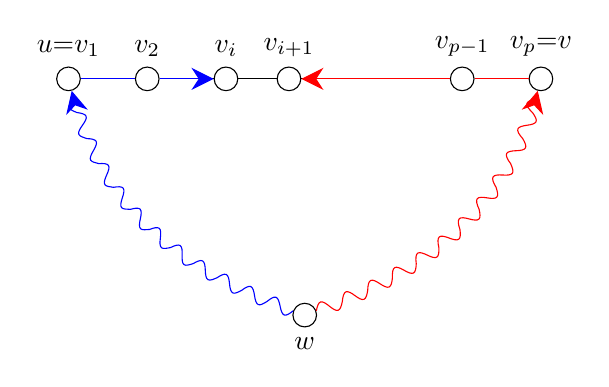
\begin{tikzpicture}
				%%%S_uv
				\node[vert,label=above:$u {=} v_1$] (v1) at (1,0) {};
				\node[vert,label=above:$v_2$] (v2) at (2,0) {};
				\node[vert,label=above:$v_i$] (vi) at (3,0) {};
				\node[vert,label=above:$v_{i+1}$] (vi+1) at (3.8,0) {};
				\node[vert,label=above:$v_{p-1}$] (vp1) at (6,0) {};
				\node[vert,label=above:$v_p {=} v$] (vp) at (7,0) {};
				\draw (v1) -- (v2) -- (vi) -- (vi+1) -- (vp1) -- (vp);
				
				%%%% node w
				\node[vert,label=below:$w$] (w) at (4,-3) {};
				
				
				
				\draw [blue] 
				(w) edge[dirwave] [out=160,in=285] (v1) 
				(v1) -- (v2)
				(v2) edge[diredge2] (vi);
				
				\draw [red]
				(w) edge[dirwave] [out=20,in=255] (vp) 
				(vp) -- (vp1)
				(vp1) edge[diredge2] (vi+1);
				
		\end{tikzpicture}}
		\caption{Example of a guess G-7, where, for a vertex of interest $w$, 
			we
			calculated its corresponding split vertex $v_i \in S_{u,v}$,
			and guessed the fastest paths of form
			$w \leadsto u \rightarrow v_2 \rightarrow \cdots \rightarrow v_i$  (in blue) 
			and $w \leadsto v \rightarrow v_{p-1} \rightarrow \cdots \rightarrow v_{i+1}$ (in red). 
			\label{fig:FPT-guessG7}}
	\end{subfigure}
	\caption{An example of guesses G-4, G-5, G-6 and G-7.}
\end{figure}


	\begin{figure}[h]
	\centering
	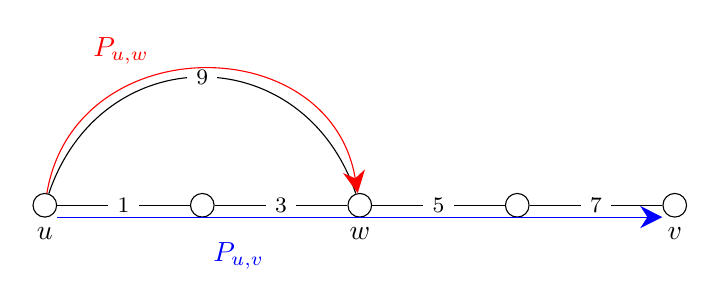
\begin{tikzpicture}[xscale=2]
		%%%S_uv
		\node[vert,label=below:$u$] (v1) at (1,0) {};
		\node[vert] (v2) at (2,0) {};
		\node[vert,label=below:$w$] (v3) at (3,0) {};
		\node[vert] (v4) at (4,0) {};
		\node[vert,label=below:$v$] (v5) at (5,0) {};
		\draw (v1) -- node[timelabel] {$1$} (v2) -- node[timelabel] {$3$}  (v3) -- node[timelabel] {$5$} (v4) -- node[timelabel] {$7$} (v5);
		\draw (v1) to [out=80,in=100,distance=2cm] node[timelabel] {$9$} (v3);
		
		\draw[transform canvas={yshift=-1.5mm}, blue]
		(v1) edge[diredge2]  node[pos=0.3,yshift=-2,label=below:$P_{u,v}$] {} (v5) ;
		
		\draw[red]
		(v1) edge[diredge2] [out=85,in=95,distance=2.1cm] node[pos=0.3,yshift=2,label=above:$P_{u,w}$] {} (v3) ;
	\end{tikzpicture}
	\caption{An example of a temporal graph, where the fastest temporal path $P_{u,v}$ (in blue) from $u$ to $v$ is of duration $7$,
		while the fastest temporal path $P_{u,w}$ (in red) from $u$ to a vertex $w$ that is on a path $P_{u,v}$ is of duration $1$ and is not a subpath of $P_{u,v}$.		
		\label{fig:ftpExample}}
\end{figure}

%
\begin{figure}[h]
	\noindent
	\makebox[\textwidth]{
		\centering
		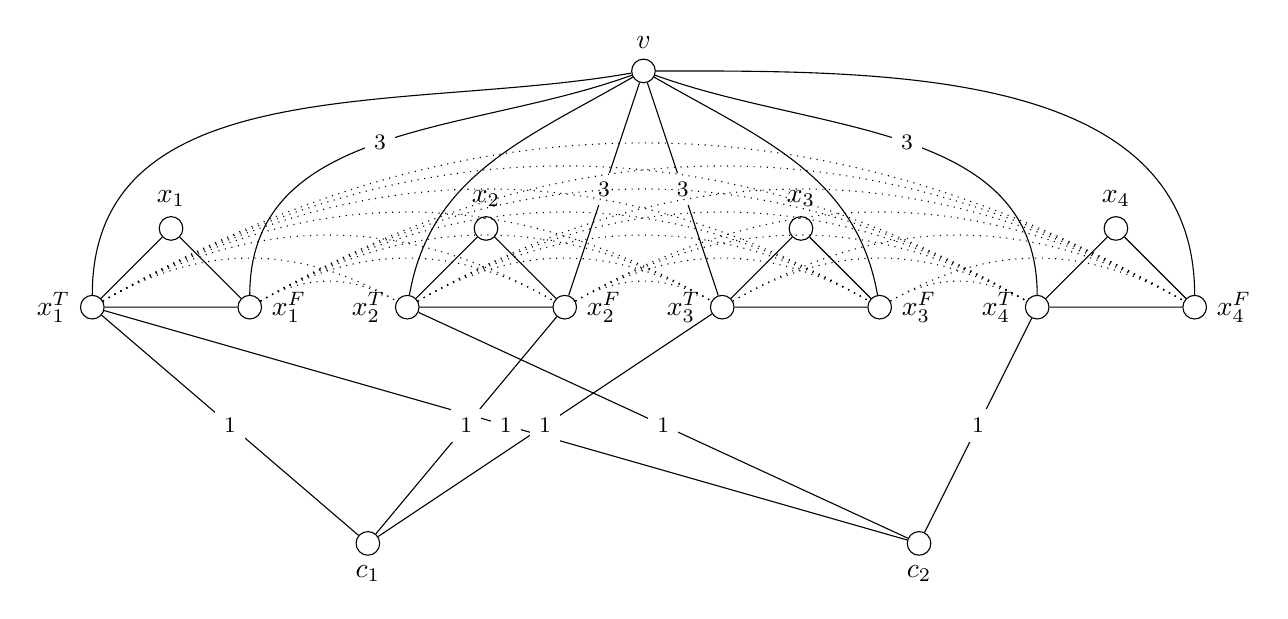
\begin{tikzpicture}%[xscale=2]
			
			%%Variable X1
			\node[vert,label=left:$x_1^T$] (x1t) at (1,0) {};
			\node[vert,label=right:$x_1^F$] (x1f) at (3,0) {};
			\node[vert,label=above:$x_1$] (x1) at (2,1) {};
			\draw (x1t) -- (x1f) -- (x1) -- (x1t);
			
			%%Variable X2
			\node[vert,label=left:$x_2^T$] (x2t) at (5,0) {};
			\node[vert,label=right:$x_2^F$] (x2f) at (7,0) {};
			\node[vert,label=above:$x_2$] (x2) at (6,1) {};
			\draw (x2t) -- (x2f) -- (x2) -- (x2t);
			
			%%Variable x3
			\node[vert,label=left:$x_3^T$] (x3t) at (9,0) {};
			\node[vert,label=right:$x_3^F$] (x3f) at (11,0) {};
			\node[vert,label=above:$x_3$] (x3) at (10,1) {};
			\draw (x3t) -- (x3f) -- (x3) -- (x3t);
			
			%%Variable x4
			\node[vert,label=left:$x_4^T$] (x4t) at (13,0) {};
			\node[vert,label=right:$x_4^F$] (x4f) at (15,0) {};
			\node[vert,label=above:$x_4$] (x4) at (14,1) {};
			\draw (x4t) -- (x4f) -- (x4) -- (x4t);
			
			%%vertices for clauses c1, c2 + vertex v
			\node[vert,label=above:$v$] (v) at (8,3) {};
			\node[vert,label=below:$c_1$] (c1) at (4.5,-3) {};
			\node[vert,label=below:$c_2$] (c2) at (11.5,-3) {};
			
			%%% edges between x1 gadget and v,c1,c2
			\draw (x1t) to node[timelabel] {$1$} (c1);
			\draw (x1t) to node[timelabel] {$1$} (c2);
			\draw (x1t) to [out=90,in=190] (v);
			\draw (x1f) to [out=90,in=200] node[timelabel] {$3$} (v);
			
			%%% edges between x2 gadget and v,c1,c2
			\draw (x2f) to node[timelabel] {$1$} (c1);
			\draw (x2t) to node[timelabel] {$1$} (c2);
			\draw (x2t) to [out=80,in=210]  (v);
			\draw (x2f) to node[timelabel] {$3$} (v);
			
			%%% edges between x3 gadget and v,c1
			\draw (x3t) to node[timelabel] {$1$} (c1);
			\draw (x3t) to node[timelabel] {$3$} (v);
			\draw (x3f) to [out=100,in=330] (v);
			
			%%% edges between x4 gadget and v,c2
			\draw (x4t) to node[timelabel] {$1$} (c2);
			\draw (x4t) to [out=90,in=340] node[timelabel] {$3$} (v);
			\draw (x4f) to [out=90,in=360] (v);
			
			%% edges among xt, xf vertices
			%x1 to all
			\draw [dotted] (x1t) [out=30,in=150] to (x2t);
			\draw [dotted] (x1t) [out=30,in=150] to (x3t);
			\draw [dotted] (x1t) [out=30,in=150] to (x4t);
			\draw [dotted] (x1t) [out=30,in=150] to (x2f);
			\draw [dotted] (x1t) [out=30,in=150] to (x3f);
			\draw [dotted] (x1t) [out=30,in=150] to (x4f);
			
			\draw [dotted] (x1f) [out=30,in=150] to (x2t);
			\draw [dotted] (x1f) [out=30,in=150] to (x3t);
			\draw [dotted] (x1f) [out=30,in=150] to (x4t);
			\draw [dotted] (x1f) [out=30,in=150] to (x2f);
			\draw [dotted] (x1f) [out=30,in=150] to (x3f);
			\draw [dotted] (x1f) [out=30,in=150] to (x4f);
			%x2 to all
			\draw [dotted] (x2t) [out=30,in=150] to (x3t);
			\draw [dotted] (x2t) [out=30,in=150] to (x4t);
			\draw [dotted] (x2t) [out=30,in=150] to (x3f);
			\draw [dotted] (x2t) [out=30,in=150] to (x4f);
			
			\draw [dotted] (x2f) [out=30,in=150] to (x3t);
			\draw [dotted] (x2f) [out=30,in=150] to (x4t);
			\draw [dotted] (x2f) [out=30,in=150] to (x3f);
			\draw [dotted] (x2f) [out=30,in=150] to (x4f);
			%x3 to all
			\draw [dotted] (x3t) [out=30,in=150] to (x4t);
			\draw [dotted] (x3t) [out=30,in=150] to (x4f);
			
			\draw [dotted] (x3f) [out=30,in=150] to (x4t);
			\draw [dotted] (x3f) [out=30,in=150] to (x4f);
		\end{tikzpicture}
	}
	\caption{Example of the temporal graph $(G_\phi,\lambda)$ from the NP-hardness reduction, 
		where the 3-SAT formula $\phi$ is of form $\phi = (x_1 \vee \overline{x_2} \vee x_3) \wedge (\overline{x_1} \vee x_2 \vee x_4)$.
		For the simplicity we draw edges between vertices $x_i^T$ and $x_j^F$ (where $i \neg j$) with a dotted line.
		Presented is the labeling of $G_\phi$, corresponding to the assignment $x_1=x_2=\textsc{True}$ and $x_3,x_4=\textsc{False}$,
		where all unlabeled edges get the label $2$.}
\end{figure}

	\begin{figure}[h]
	\centering
	\begin{tikzpicture}[xscale=1.3]
		%%%S_uv
		\node[vert,label=below:$u{=} v_1$] (v1) at (1,0) {};
		\node[vert, label=below:$v_2$] (v2) at (2,0) {};
		\node[vert,label=below:$v_3$] (v3) at (3,0) {};
		\node[vert,label=below:$v_{i-1}$] (vi-1) at (6,0) {};
		\node[vert,label=below:$v_i$] (vi) at (7,0) {};
		\node[vert,label=below:$v_{i+1}$] (vi+1) at (8,0) {};
		\node[vert,label=below:$v_{p} {=} v$] (v) at (10,0) {};
		
		
		\draw (v1) -- node[label={above:$t_{v_2}$},yshift=-5] {} (v2) -- (v3) -- (vi-1) -- node[label={above:$e$},yshift=-5] {} (vi) -- node[label={above:$f$},yshift=-5] {} (vi+1) -- (v);
		
		\draw (v1) edge[bend left=80,distance=3cm]
		node[pos=0.1,label={left:$t_{u_2}$}] {}
		node[vert,pos=0.15,label=above:$u_2$] {}
		node[vert,pos=0.3,label=above:$u_3$] {}
		node[vert,pos=0.85,label=above:$u_{j-1}$] {}
		node[pos=0.9,label={right:$g$}] {} (vi);
		
		%\draw[edge] (v1)  edge[bend right=80,distance=3cm]  (vi);
		
		%\draw[transform canvas={yshift=0mm}, blue]
		%(v1) -- (v2) -- (v3) -- node[pos=0.3,yshift=-2,label=above:$P_{u,v}$] {} (vi-1) -- (vi) ;
		
		%\draw[red]
		%(v1) edge[diredge2] [out=85,in=95,distance=2.1cm] node[pos=0.3,yshift=2,label=above:$P_{u,w}$] {} (v3) ;
	\end{tikzpicture}
	\caption{An example of the situation in %\cref{lemma:FPT-uv-LabelAlmostalledges},
		where we assume that the fastest temporal path from $u$ to $v$ is $P_{u,v} = (u=v_1, v_2, \dots v_p)$,
		and the fastest temporal path from $u$ to $v_i$ in $P_{u,v}$ is $P = (u, u_2, u_3, \dots, v_i)$.
		We denote with $Q = (u=v_1, v_2, \dots, v_i)$ and with $R = (v_i, v_{i+1}, \dots, v_p=v)$.
		\label{fig:FPT-uv-Labelalledges}}
\end{figure}


\end{document}